% TODO: scrivere discussione dello schema ER portante
% DONE: definire schema ER portante
\section{Schema E/R portante}
\begin{figure}
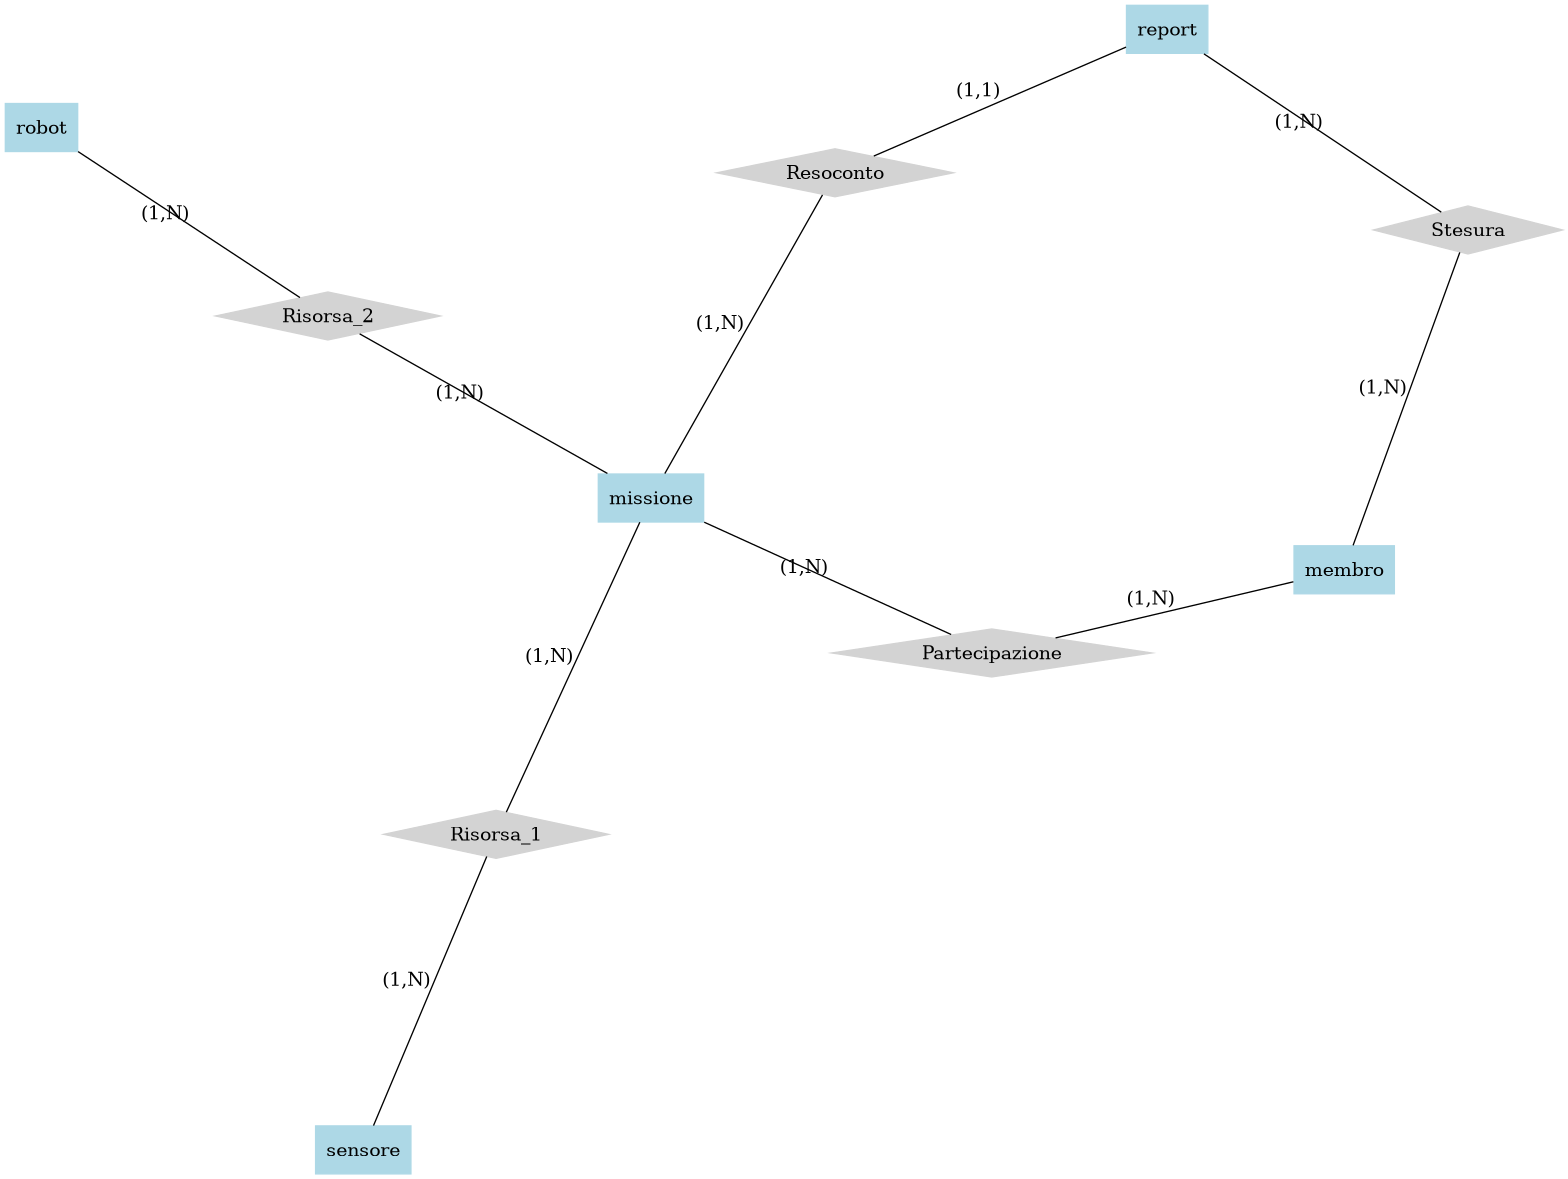
\includegraphics[width=\linewidth]{images/er-portante.png}
\caption{Modello E/R portante per \texttt{ASTRADM}}
\label{fig:er-portante}
\end{figure}           
Analizzando le problematiche presentate si è arrivati all'individuazione delle
seguenti entità fondamentali:
\begin{description}
\item[Membro] 
\item[Missione]
\item[Report]
\item[Robot]
\item[Sensore]
\end{description}
Come visibile da \ref{fig:er-portante}

